%\documentclass{article}
\documentclass[preprint,aip,cha]{revtex4-1}
\usepackage{hyperref}
\usepackage{amsmath}
\usepackage{graphicx}
\graphicspath{ {images/} }
\usepackage{physics}
\usepackage{float}
\usepackage{color}
\newcommand{\red}[1]{\textcolor{red}{#1}}

\begin{document}

\section{Introduction}
IAEA nuclear waste estimation: over 1000 tons of highly radioactive waste.\cite{iaea08}
Nuclear power estimate:increase by 40\% by 2020. \cite{iaea12}
meep. Mostly focus on nuclear waste from reactors.
global policy review \cite{r12} 
\begin{itemize}
    \item history
    \item nuclear decay mechanism: weak force and tunnelling, radioactive decay
    \item reactors?
    \item What is nuclear waste and why is it harmful?
    \item partition and transmutation
    \item Above-ground disposal: look at sites, dry-casks storage
    \item geological disposal ($\star$), Yucca mountain as an example
    \item ocean floor disposal which was done by everyone but not legal any more
    \item transmutation
    \item todo: find sources on the specific health impact of nuclear waste instead of radiation
        in general
\end{itemize}

\section{Nuclear Physics}
    Three principle prossess happen in a reactor: scattering, radiative capture and fission.
    In each of these processes neutrons are involved.
    \subsection{Radioactivity(and how to quantify it)}
        \subsubsection{Quantum Theory of Radioactive decays}
        some QM to explain nuclear excitation and ways to change into more stable system.
        nuclear instability
    \subsection{Properties of a neutron}
        Because neutron plays a central role in the physical processes taking
        place in a recator, we should first look at some of its
        properties. A free neutron has a half-life of about $10.2$ minutes. \cite{gc01} The Standard
        Model dictates that a free neutron can only go through beta decay, in which a neutron decays
        into a proton, an electron, and an electron antineutrino \red{(source)}. The decay can be denoted by
        \[n^0 \rightarrow p^+ + e^- + \bar{\nu}_e,\]
        where $n$ denotes a neutron, $p^+$ a proton (that is positively charged), $e^-$ a
        (negatively charged) electron and $\bar{\nu}_e$ an electron antineutrino.

        While a free neutron decays relatively quickly, a neutron bound to a proton is usually stable.
        A neutron may go through beta decay in an unstable nucleus formed by neutrons and protons(\red{more}). 

        A neutron can also be captured by a nucleus as it travels through materials. Since a neutron is neutrally
        charged, it requires much less energy to combine with a nucleus than does
        an alpha particle since it does not experience the Coulumb barrier.
        Neutron capture usually produces a neutron that is unstable and thus
        more radioactive than the stable nucleus found in nature.

    \subsection{Neutron Capture}
        \red{cross section?}
    \subsection{Fission}
        \subsubsection{Fission and fission products}
        Conjectured by Bohr and proven by Alfred O. Nier in 1939,
        the fission of uranium-235 induced by a thermal neutron
        is the best-known example of induced fission. 
        The neutron capture produces a compound nucleus ${}^{236}U$ that is in an excited state.
        Sometimes the nucleus can decay by $\gamma$ emission in capture reaction. \red{(?)}
        But most of the time, the excitation energy deforms the nucleus (see Figure \ref{fig:fission}).
        When the
        deformation reaches a certain point, the Coulumb force overcomes the short-ranged nuclear
        force (residual strong force) and the nucleus disintegrate into two large fragments and several neutrons. The
        positively-charged fragments(fission products) attain approximately $170$ MeV of kinetic energy as
        Coulumb force continues to drive them apart.\cite{l01}
        A typical reaction is described by
        \[{}^{235}_{92}\text{U} + n \rightarrow {}^{92}_{36}\text{Kr} + {}^{142}_{56}\text{Ba} + 2 n.\]
        The energy liberated is about $180$ MeV. The combination of fission products is not
        unique. \cite{w98, gc01}
        Very often, photons, electrons and nutrinos are also emitted through beta and gamma decay.
        \red{(insert 10.2 from Lilley here? distribution of fission fragment masses)}
        Radioactive if neutron-to-proton ratio is over 5. On average, $2.5$ neutrons are produced per fission.\cite{l01} 
        \begin{figure}[H]
            \centering
            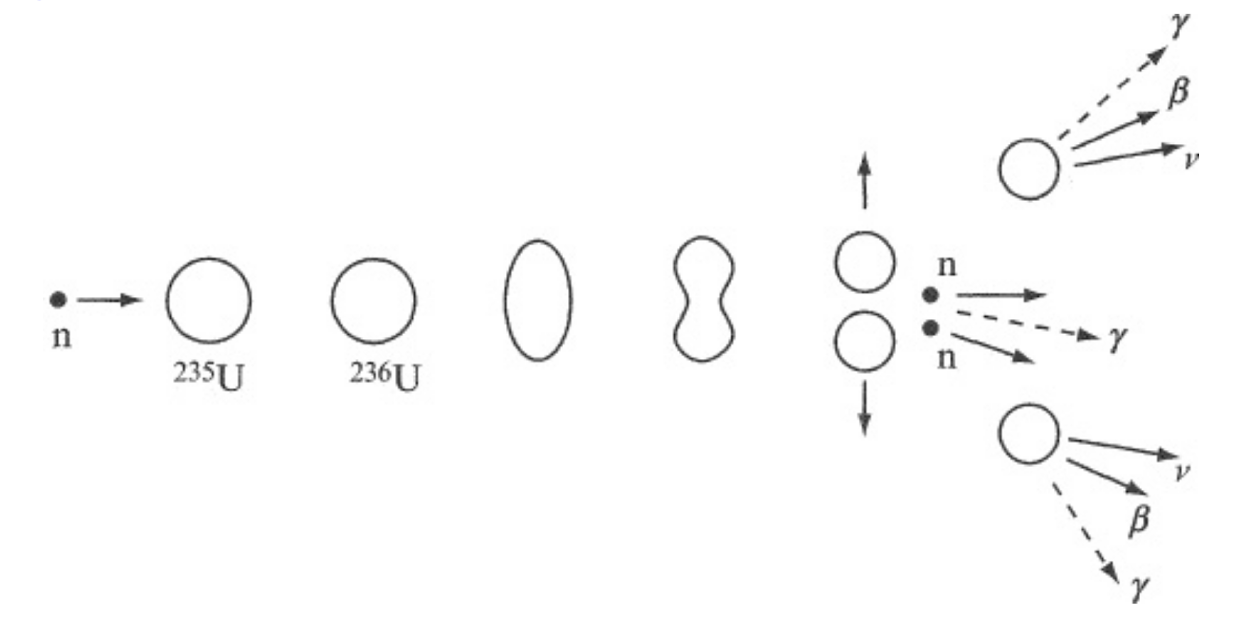
\includegraphics[width=0.8\textwidth]{fission.png}
            \caption{Illustration of the fission process for uranium-235.\cite{l01}}
            \label{fig:fission}
        \end{figure}

        \subsubsection{Fission energy budget}
        We can estimate the amount of energy released in fission by considering the binding energy difference
        and the properties of the product.
        The binding energy per nucleon is about $7.6$ MeV u${}^{-1}$ for uranium and about $8.5$ MeV u${}^{-1}$
        for a nucleus with atomic number around $117$. Hence, the change of binding energy per nucleon is
        $0.9$ MeV u${}^{-1}$, which amount to $212$ MeV for uranium-235.
        About $87\%$ of the total energy is promptly emitted because
        the fission products, carrying over $90\%$ of the total energy, travel for only a fraction of a
        millimeter before they are stopped. Besides, fission neutrons emit about $2$ MeV of energy by
        successive scattering in the reactor.
        About $13\%$ of the total energy goes into radioactivity. Energy carried by electrons and photons is
        convertible to heat but the nutrinos, carrying about $50\%$ of the radiation energy, are not stoppable.

        Henceforth, it is generally accepted that about $220$ MeV per fission is recoverabe for energy conversion.
        This is about 2.5 million times the energy produced by burning coal of the same mass.\cite{e17}
        \subsubsection{Chain reaction??}

\section{Effect of Radiation on Human}
    meep

\section{Formation of (High-Level) Nuclear Waste}
    The IAEA classifies nuclear waste by considering the activity content and the half-life
    of the radionuclides (see Figure \ref{fig:scheme}). Activity content is a measure of how much nuclear activity
    a given amount of wastes contain: a form of waste may possesses a high activity content due to
    a high concentration or high activity.\cite{iaea09}
    \begin{figure}[H]
        \centering
        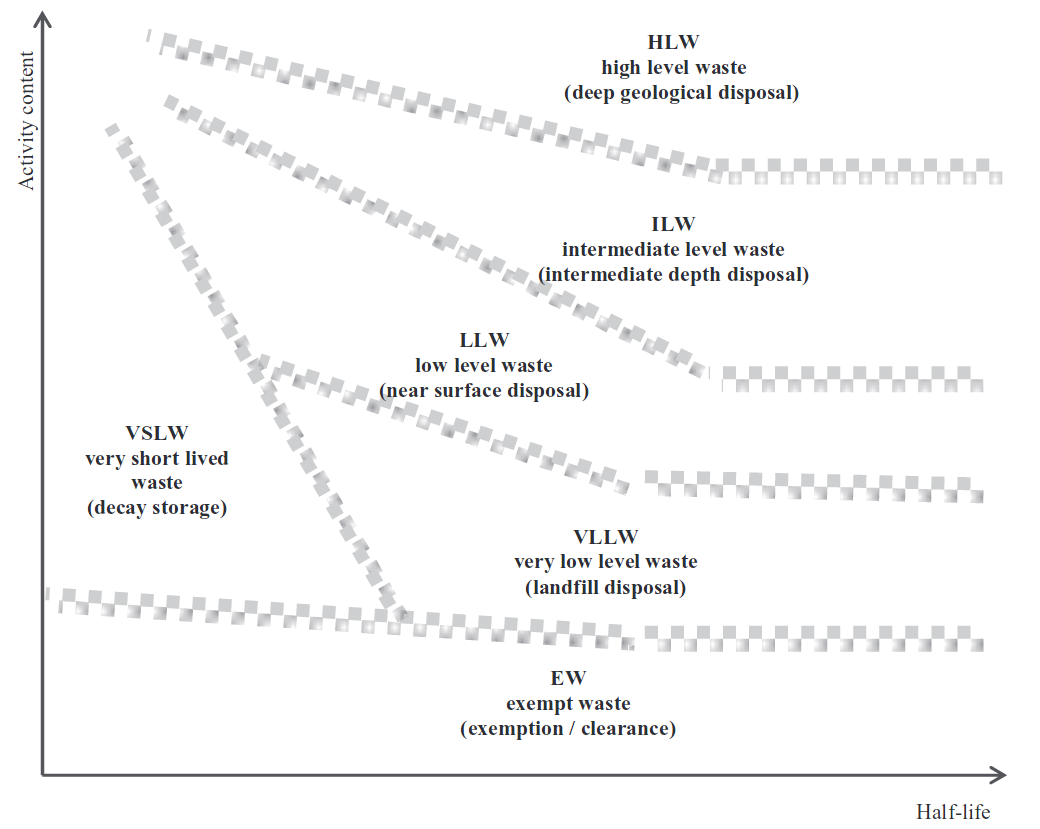
\includegraphics[width=0.7\textwidth]{wastescheme.png}
        \caption{An illustration of the IAEA classification scheme for nuclear wastes.\cite{iaea09}}
        \label{fig:scheme}
    \end{figure}

    High-level Wastes (HLW) are highly radioactive and usually
    hot. The typical source of HLW is spent fuel from the nuclear reactor. In a nuclear reactor,
    fission of uranium-235 produces lighter radionuclides like cesium-137 and strontium-90, which
    account for most of the heat and penetrating radiation (\red{penerating?}). In addition to
    the fission process, some uranium-235 atoms go through neutron capture and produce elements that are
    heavier than uranium ("transuranic") such as plutonium. The transuranic atoms do not generate
    as much heat or radiation as the fission products, but they tend to have a much longer half-life.
    For example, strontium-90 and cesium-137 have half-lives of about $30$ years, whereas
    plutonium-239 has a half-life of $24,000$ years. https://www.nrc.gov/reading-rm/doc-collections/fact-sheets/radwaste.html
    \red{transition needed}

    \subsection{Fission products}
    meep
    \subsection{Transuranic radionuclides}
    mop
    \subsection{Trade-offs}
    short huge dose or long small dose?

\section{Impacts}

\section{Disposal}


\section{Nuclear Decay}
k
\begin{acknowledgments}
Thanks Joel and peeps. Arjendu and M. V. Ramana.
\end{acknowledgments}

\pagebreak
\bibliographystyle{aip}
\bibliography{refs}
\end{document}
